\documentclass{article}
\title{Notes for ECE 2714}
\author{C.L. Wyatt}

% Document Formatting
\usepackage[letterpaper, margin=1in]{geometry}

% Configure Math
\usepackage{amsmath}
\usepackage{amssymb}

% Configure graphics
\usepackage{graphicx}

\begin{document}
\maketitle
\newpage

\tableofcontents
\newpage

% switch formatting
\setlength{\parindent}{0em}
\setlength{\parskip}{1em}

\section{Course Introduction}
\label{sec:intro}
\begin{itemize}
\item Course Overview
\item Learning Objectives, reinterpret for them as "big ideas"
\item Schedule and Course Activities
\item Grading
\end{itemize}

\newpage
\section{Prerequisites}

This course uses many concepts from prerequisite courses, particularly those from calculus and circuits. While we assume you know this material, the following sections offer a review of the most pertinent and establish some notation. If you have trouble with any of them seek assistance -- the sooner the better.

\subsection{Complex Numbers}

Complex numbers are used extensively throughout the course. You need to be very adept at manipulating them.

\subsubsection{The Number System}

By way of review and to motivate the discussion of complext numbers, recall the following basic facts.

\begin{itemize}
\item The \emph{Natural Numbers} $\mathbb{N}$ are the positive integers $1,2,3,4,\cdots$. Given two natual numbers $a$ and $b$ the sum $a+b$ and the product $a\,b$ are also natural numbers, that is the set of natural numbers is \emph{closed} under addition and multiplication.

\item Solving equations of the form $x + a = b$ for any natural numbers $a,b$ requires the introduction of the negative integers $\cdots, -4, -3, -2 -1$ and $0$. These plus the natural numbers give the \emph{integers}  $\mathbb{Z}$. Note $\mathbb{N} \subset \mathbb{Z}$. Zero ($0$) is called the identity element with respect to addition, while $1$ is the identity with respect to multiplication, that is $a+0 = a$ and $ a \cdot 1 = a$. The \emph{inverse} of an integer $a$ is $-a$, such that thier sum gives the identity for addition, i.e. $a + -a = 0$.

\item The \emph{rational numbers} $\mathbb{Q}$ are of the form $\frac{b}{a}$ for integers $a,b$ with $a \neq 0$. They solve problems of the form $ax=b$ and provide the inverse for multiplication since $\frac{1}{a} \cdot a = 1$. Note $\mathbb{Z} \subset \mathbb{Q}$

\item The \emph{irrational numbers} are those that cannot be written as a rational number, for example $\sqrt{2} = 1.414\ldots$ and $\pi = 3.14159\ldots$

\item The union of the rational and irrational numbers give the \emph{real numbers} denoted $\mathbb{R}$.
\end{itemize}

Graphically the numbers and thier ordering can be expressed using the number line:

\begin{center}
  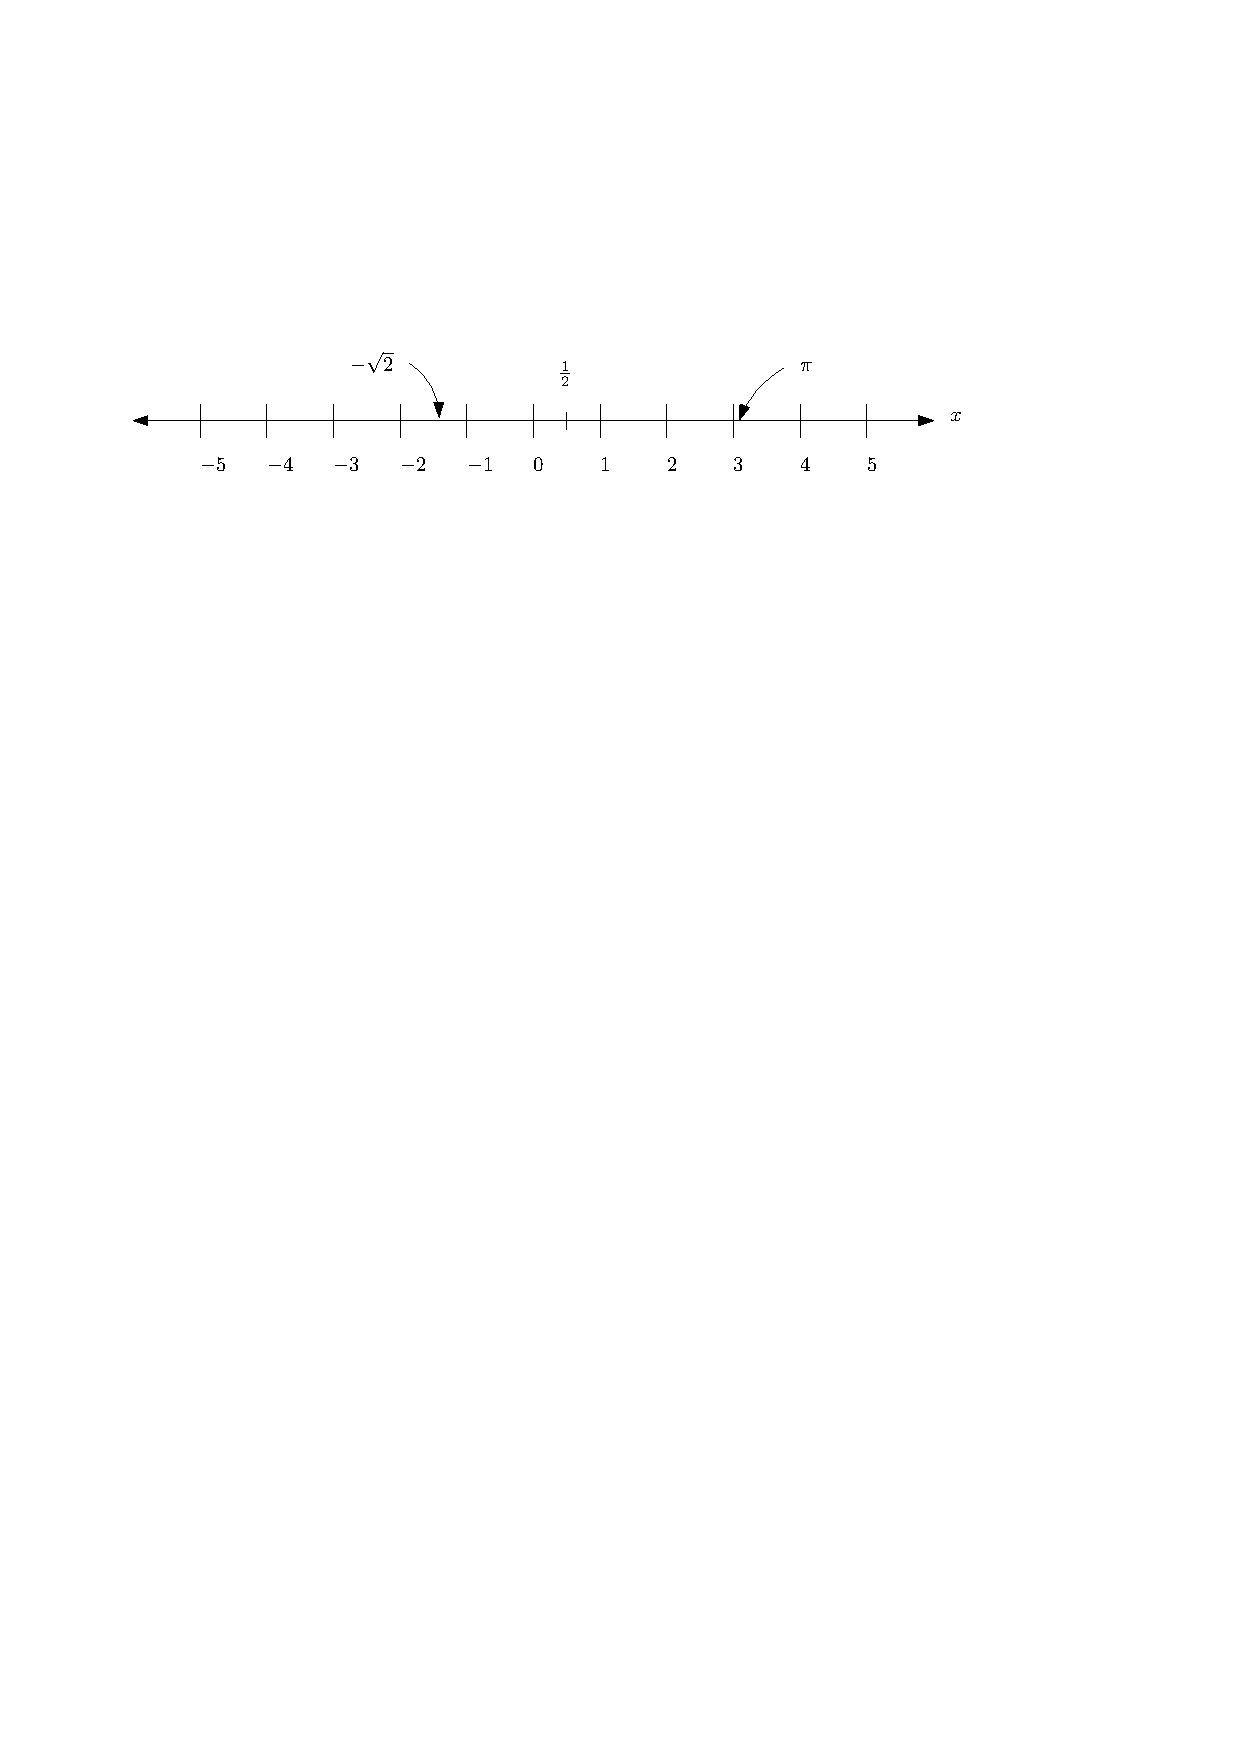
\includegraphics[scale=1]{graphics/number-line.pdf}
\end{center}

\subsubsection{Complex numbers as extension of reals}

Continuing the pattern of the basic number system we can ask what are solutions of equations of the form $x^2+a = 0$ or $x^2 + 2ax +a^2 + b^2 = 0$ for $a,b \in \mathbb{R}$ ? As above, finding such solutions requires moving to a larger set of numbers, the \emph{complex numbers} denoted $\mathbb{C}$.

A complex variable $z\in\mathbb{C}$ can be written as $z = a + j\, b$ for $a,b\in\mathbb{R}$, where $j$ is the imaginary unit and $j^2 = -1$. Note in mathematics the imaginary unit is denoted $i$; this difference is purely historical. 

\begin{itemize}
\item the \emph{real part} $\Re(z) = \text{Re}(z) = a$
\item the \emph{imaginary part} $\Im(z) = \text{Im}(z) = b$
\item two complex numbers $z_1, z_2\in \mathbb{C}$ are equal if $\text{Re}(z_1) = \text{Re}(z_2)$ and $\text{Im}(z_1) = \text{Im}(z_2)$
\item $\mathbb{R} \subset \mathbb{C}$, when $b = 0$ and we say that the number is purely real
\item if $a = 0$ we say the number is purely imaginary
\item the \emph{complex conjugate} of $z = a + jb$ is $z^* = a - jb$.
\end{itemize}

\subsubsection{Operations}


\subsubsection{Absolute Value (Magnitude)}

\subsubsection{Complex numbers as ordered pair}

\subsubsection{Basic properties}

\begin{itemize}
\item equality
\item sum
\item product
\item closure
\item communative law of addition and multiplication
\item associative law of addition and multiplication
\item idenity elements 0 and 1
\item inverse -z and 1/z
\end{itemize}
\subsubsection{Graphical representation of complex numbers}

TODO: Visualization of multiplication by j.

\subsubsection{Polar representation of complex numbers, Magnitude an Phase}

\subsubsection{De Moivre's Theorem}

\subsubsection{Roots and powers of complex numbers}

\subsubsection{Euler's formula}

\subsubsection{Complex numbers as roots of polynomial equations}

\subsubsection{The nth roots of unity}

\subsubsection{Vector interpretation of complex numbers}

\subsection{Calculus}

\subsubsection{Functions}

\begin{itemize}
\item $f:\mathbb{R}\mapsto\mathbb{R}$
\item $f:\mathbb{R}\mapsto\mathbb{C}$
\end{itemize}

\subsubsection{Review derivative}

\subsubsection{Review Reimann integral}

Complex integrals?

\subsubsection{Numerical approximations?}

\subsection{Complex valued functions}

\subsubsection{functions from reals to complex}

\subsubsection{derivatives of such functions}

\subsubsection{integrals of such functions}

\subsubsection{Magnitude and Phase representation of such functions}

\subsection{Differential Equations}

\subsubsection{linear, constant-coefficient differential equations, homogeneous and particular solutions}

\subsection{Circuits}

\subsubsection{KVL}

\subsubsection{KCL}

\subsubsection{Ideal OpAmps}

\subsubsection{from circuit to differential equation}

\subsubsection{using LiaB and building/measuring circuits}

\subsection{Programming}

\subsubsection{plotting and vizualization with Matlab/Python/Julia}

\subsubsection{Computation with C or C++}

\subsection{Digitial Systems}

\subsubsection{binary representation of integers vs floating point}

\subsubsection{shift registers}

\subsubsection{adders and multipliers}

\newpage
\section{CT and DT Signals}
\label{sec:org3203c88}
\subsection{What are signals models and what are they good for}
\label{sec:orga6591cb}
\subsection{Continuous-Time (CT) Signals as functions}
\label{sec:org6225bd5}
\subsection{Discrete-Time (DT) Signals as functions}
\label{sec:orga54c05e}
\subsection{Building signal models from primitives}
\label{sec:org08f49f3}
\subsection{Examples}
\label{sec:orgf29c95e}

\newpage
\section{Signal Transformations}
\label{sec:org6555689}
\subsection{scaling DT and CT signals}
\label{sec:org0fa5a47}
\subsection{derivatives and integrals of CT signals}
\label{sec:orgb56c3af}
\subsection{backward/forwrd differences and running sums of DT signals}
\label{sec:orgcb4a125}
\subsection{sums of signals, foreshadow CTFS and DTFS}
\label{sec:orge4464f9}
\subsection{multiplication (modulation)}
\label{sec:orgc1443f6}
\subsection{Transformations of Time / Index}
\label{sec:orgb786926}
\begin{itemize}
\item time shift, forward and backward
\item index shift, forward and backward
\item time reversal
\item index reversal
\item time scaling
\item index decimation and interpolation
\end{itemize}

\newpage
\section{Signal Characterization}
\label{sec:org122fb16}
\subsection{periodic signals}
\label{sec:org5c7f0c9}
\subsection{even/odd signals}
\label{sec:org4721db8}
\subsection{Signal Energy and Power of CT Signals}
\label{sec:org177586b}
\subsection{Signal Energy and Power of DT Signals}
\label{sec:orgc0bedd6}

\newpage
\section{Exponential and Sinusoidal Signals}
\label{sec:orge17b3c1}
\subsection{complex exponential signals in CT and DT}
\label{sec:org9255270}
\subsection{special case of sinusoids}
\label{sec:orgecba192}
\subsection{harmonics}
\label{sec:org5e8d9ab}
\subsection{properties of sinusoids}
\label{sec:orga96306e}
\subsection{interpreting sinusoids from plots/traces}
\label{sec:org53b2fa0}
They need to be able to read off the magnitude and phase and convert the phase to a time shift. Many struggle with this basic skill.

\newpage
\section{The Unit Impulse Functions}
\label{sec:org33257b0}
\subsection{DT impulse}
\label{sec:org1210e0d}
\subsection{CT impulse}
\label{sec:org5a0b8cc}

\newpage
\section{The Unit Step Functions}
\label{sec:orgcd386ae}
\subsection{DT step}
\label{sec:org0ecc466}
\subsection{CT step}
\label{sec:org4d099d0}
\subsection{relationship between impulse and step}
\label{sec:org055e977}

\newpage
\section{CT and DT Systems}
\label{sec:org7f962be}
\subsection{Models of systems and what they are good for}
\label{sec:org630c08b}
\subsection{Definition of CT systems}
\label{sec:org4c0c08a}
\subsection{Definition of DT systems}
\label{sec:org93604c1}
\subsection{Examples: Circuits}
\label{sec:org787bf61}
\subsection{Basic block diagram representation}
\label{sec:orgb2e3c34}

\newpage
\section{Basic System Properties}
\label{sec:org4a5eb76}
\subsection{Memory}
\label{sec:org11a1ea9}
\subsection{Invertability}
\label{sec:org73bcf64}
\subsection{Causality}
\label{sec:org4314405}
\subsection{Stability}
\label{sec:orgdf1ed25}
\subsection{Time-invariance}
\label{sec:org0eb860c}
\subsection{Linearity}
\label{sec:org07e3ada}
\subsection{Define LTI system}
\label{sec:org920390a}

\newpage
\section{Convolution}
\label{sec:org9c1558d}
\subsection{Review LTI systems and superposition property}
\label{sec:orgc9b2a56}
\subsection{DT Convolution Sum}
\label{sec:org9ec80b8}
\subsection{CT Convolution Integral}
\label{sec:orge42c03e}
\subsection{Properties of convolution}
\label{sec:orgbed0c56}

\subsubsection{Convolution is commutative}

In DT: $x_1[n] * x_2[n] = x_2[n] * x_1[n]$


In CT: $x_1(t) * x_2(t) = x_2(t) * x_1(t)$


Thus the system response can be viewed as the convolution of input with impulse response (e.g. in DT)
    \[
      y[n] = \sum\limits_{k=-\infty}^{\infty} x[k]h[n-k] = x[n] * h[n]
    \]
    or, convolution of impulse response with the input
    \[
      y[n] = \sum\limits_{k=-\infty}^{\infty} h[k]x[n-k] = h[n] * x[n]
    \]

  One way is sometimes more mathematically convenient than the other.
  
  \subsubsection{distributive}
  
\subsubsection{associative}
\subsubsection{how they apply to block diagrams}

\newpage
\section{Properties of LTI Systems}
\label{sec:orgdadbbac}
\subsection{Memory}
\label{sec:org3a53807}
\subsection{Invertable}
\label{sec:orgeec0268}
\subsection{causal}
\label{sec:orgdb3dd89}
\subsection{BIBO stability}
\label{sec:org59a881d}

\newpage
\section{Systems as Differential and Difference Equations}
\label{sec:orgc840576}
\subsection{LCC differential equations and thier solution}
\label{sec:org8004f54}
\subsection{impulse response from LCC differential equation}
\label{sec:org808b8e9}
\subsection{LCC difference equations and their solution}
\label{sec:org17be1e7}
\subsection{impulse response from LCC difference equation}
\label{sec:org96b828a}

\newpage
\section{Block Diagram continued}
\label{sec:orgcb5c75f}
\subsection{equivalence of LCCDE's and clock diagrams}
\label{sec:org36f6bc1}
\subsection{firt-order difference equation as feedback motif}
\label{sec:orgd43ce46}
\subsection{implementing a difference equation using adders, multipliers, and delays}
\label{sec:org7e3b256}
\subsection{second-order difference equation implementation}
\label{sec:org86279c9}
\subsection{first-order differential equation as feedback motif}
\label{sec:org3fcff6e}
\subsection{implementing a differential equation using adders, multipliers, and integrators}
\label{sec:org60f5c97}
\subsection{second-order differential equation as a feedback motif}
\label{sec:orgcc26b56}

\newpage
\section{Unit Impulse Revisited}
\label{sec:org9c858ee}
\subsection{Intuition about the impulse response}
\label{sec:org8432368}
\subsection{decomposition into scaled-shifted impulse functions}
\label{sec:org23917a7}
\subsection{why convoluton gives the response desired}
\label{sec:org7ad3b62}

\newpage
\section{The Response of LTI Systems to Complex Exponentials}
\label{sec:org0d3d3bf}
\subsection{Response of CT LTI system to a complex exponential -> Transfer Function}
\label{sec:orgee51d0b}
\subsection{Response of DT LTI system to a complex exponential -> Transfer Function}
\label{sec:org7ba724a}
\subsection{How this is useful - decomposition of input signal into complex exp}
\label{sec:orge0520a1}
\subsection{What signals can be decomposed this way, foreshadow Fourier}
\label{sec:org097310e}
\subsection{Frequency response, scaling of magnitude and phase}
\label{sec:org9ebea42}

\newpage
\section{Fourier Series Representation of CT Periodic Signals}
\label{sec:org651d66d}
\subsection{review periodic functions}
\label{sec:org5c98599}
\subsection{demo/example of harmonic sums}
\label{sec:orgdc9161b}
\subsection{derive synthesis equation}
\label{sec:org9d67cc2}
\subsection{derive analysis equation}
\label{sec:org186dd6d}
\subsection{spectrum plots}
\label{sec:orgea0d486}
\subsection{examples}
\label{sec:orgda563b3}

\newpage
\section{Convergence of the Fourier Series}
\label{sec:org0a6d2d4}
\subsection{the synthesis equation is an approximation strictly speaking}
\label{sec:orge86364a}
\subsection{define mean-square convergence}
\label{sec:org992f2f9}
\subsection{truncated CT FS}
\label{sec:org1a31840}
\subsection{example, e.g. square wave as number of terms increases -> ringing}
\label{sec:org5b9a020}
\subsection{formal Dirichlet conditions}
\label{sec:orgd932eed}
\subsection{exmple of the impulse train}
\label{sec:org01d1aa2}
\subsection{practical uses of the CT Fourier series, examples}
\label{sec:org9bb1861}
\subsection{alternate forms of CTFS, trig form, compact trig form, and exp form}
\label{sec:org1f25d25}
\subsection{visualization of the CTFS as chains of rotating vectors, demo}
\label{sec:org969c81d}

\newpage
\section{Properties of CT Fourier Series}
\label{sec:org1620a4a}
\subsection{Linearity}
\label{sec:org85da9b6}
\subsection{Time shifting}
\label{sec:org39878bc}
\subsection{Time Reversal}
\label{sec:org60b9699}
\subsection{Time Scaling}
\label{sec:org69c6034}
\subsection{Multiplication}
\label{sec:orgea601f0}
\subsection{Conjugate symmetry}
\label{sec:org2c7c125}
\subsection{Parseval's}
\label{sec:orgdaf814a}

\newpage
\section{Fourier Series Representation of DT Periodic Signals}
\label{sec:org562e005}
\subsection{review CTFS and decomposition problem soving analysis}
\label{sec:org707998e}
\subsection{review DT sinusoids}
\label{sec:org5d5a23f}
\subsection{derive synthesis equation}
\label{sec:orgf946aaa}
\subsection{derive analysis equation}
\label{sec:orgf89f55d}
\subsection{spectrum plots}
\label{sec:org4f1a797}
\subsection{examples}
\label{sec:org95c7e81}

\newpage
\section{Properties of DT Fourier Series}
\label{sec:org7340971}
\subsection{linearity}
\label{sec:orga5b5f77}
\subsection{index shifting}
\label{sec:org1c757d9}
\subsection{frequency shift}
\label{sec:org4fedcd7}
\subsection{conjugation}
\label{sec:org9ab6428}
\subsection{time reversal}
\label{sec:org31bf958}
\subsection{convolution}
\label{sec:orgdefee2c}
\subsection{multiplication}
\label{sec:orge18d485}
\subsection{real signals and even/odd symmetry of coefficients}
\label{sec:org836e5ec}
\subsection{Parsevals}
\label{sec:org701c799}

\newpage
\section{Fourier Series and LTI Systems}
\label{sec:org292ffbc}
For stable, LTI systems, the frequency response scales and phase shifts each term of the series
\section{CT Filtering and Differential Equations}
\label{sec:orgf36132d}
\subsection{CT frequency response as suppressing or enhancing signal components}
\label{sec:org6a27264}
\subsection{4 basic filter types - ideal and practical frequency response}
\label{sec:orgb1ed6ac}
\subsection{simple examples: RC, CR}
\label{sec:org0734828}

\newpage
\section{DT Filters Described by Difference Equations}
\label{sec:org2b6b730}
\subsection{IIR filters and recurrence relations}
\label{sec:org928ff1a}

\subsection{FIR filters}
\label{sec:org15ab380}

\subsection{examples of both}
\label{sec:orgbb45d7e}

\newpage
\section{The CT Fourier Transform}
\label{sec:org76eb4f9}

\subsection{derive the CTFT pair from the CTFS}
\label{sec:orgdf07b5a}

\subsection{Dirichlet existance conditions}
\label{sec:org6311427}

\subsection{Examples}
\label{sec:org126acc4}

\subsection{CTFT of the CTFS}
\label{sec:orga61d23b}

\newpage
\section{Properties of the CT Fourier Transform}
\label{sec:org15bd740}

\subsection{Linearity}
\label{sec:org21f9e2d}

\subsection{Time shift}
\label{sec:orgef4cf09}

\subsection{Conjugacy}
\label{sec:org9c26c6c}

\subsection{Integration and Differentiation}
\label{sec:org8e416a7}

\subsection{Time scaling}
\label{sec:org53b0fa4}

\subsection{Duality}
\label{sec:org4485cab}

\subsection{Convolution}
\label{sec:orgf984e94}

\subsection{multiplication/modulation}
\label{sec:org7b3d857}

\subsection{Application of the properties in combination}
\label{sec:orgdb2f8f1}

\newpage
\section{Frequency Response from LTI Differential Equation}
\label{sec:org5067cc8}

\subsection{Demonstrate using the derivative property to obtain the freq response}
\label{sec:org1f03a18}

\newpage
\section{Bode plots}
\label{sec:orgb48b8af}

\subsection{why plot it this way and how to read them (not construct them manually)}
\label{sec:org340c150}

\subsection{Bode Plots in software, e.g. Matlab/Python/Julia}
\label{sec:org379a762}

\newpage
\section{The DT Fourier Transform}
\label{sec:org28dd76b}

\subsection{derive the DTFT from DTFS}
\label{sec:orge003b7a}

\subsection{examples}
\label{sec:orgc5187e0}

\subsection{DTFT of DTFS}
\label{sec:orgae5f02f}

\newpage
\section{Properties of the DT Fourier Transform}
\label{sec:org4b60654}

\subsection{periodicity}
\label{sec:org561e56c}

\subsection{linearity}
\label{sec:org77a7f35}

\subsection{index-shift}
\label{sec:org31f43b8}

\subsection{frequency shift}
\label{sec:org52b250f}

\subsection{conjugation}
\label{sec:orgfd0a284}

\subsection{finite difference and accululation}
\label{sec:orgf78b609}

\subsection{interpolation /index expansion}
\label{sec:orge721dbd}

\subsection{frequency differentiation}
\label{sec:orgf122f6b}

\subsection{Parseval's}
\label{sec:orge091617}

\subsection{convolution}
\label{sec:orgd4030e8}

\subsection{multiplication/modulation}
\label{sec:org290cfde}

\subsection{application of the proiperties in combintation}
\label{sec:orgb8ac360}

\newpage
\section{Frequency Response from LTI Difference Equation}
\label{sec:org9ac773f}

\subsection{Demonstrate using the difference property to obtain the freq response}
\label{sec:org806c699}

\newpage
\section{Magnitude-Phase Representation of the Frequency Response}
\label{sec:org24cb5f9}

\subsection{frequency resonse acting on sinusoids}
\label{sec:org1c9e86b}

\newpage
\section{Frequency-Selective Filters}
\label{sec:org81f7538}

\subsection{ideal low-pass}
\label{sec:orgcbfe22d}

\subsection{ideal high-pass}
\label{sec:org6e357c1}

\subsection{ideal bandpass}
\label{sec:orgc658523}

\subsection{ideal notch/bandstop}
\label{sec:org55a34c1}

\newpage
\section{First and Second Order Systems}
\label{sec:org9c7c5a8}

\subsection{CT 1st order RC+buffer}
\label{sec:orgdaf03e4}

\subsection{CT Sallen-key}
\label{sec:orge746d43}

\subsection{DT implementations: micro-controllers versus DSP architectures}
\label{sec:org79ad593}

\newpage
\section{The Discete Fourier Transform}
\label{sec:org2209ae0}

\subsection{time window the DTFT to get the DFT}
\label{sec:org63dec5a}

\subsection{zero-padding}
\label{sec:org07d79db}

\subsection{offline or batched filtering using the DFT}
\label{sec:orge67491a}

\subsection{briefly mention fast algorithms to compute the DFT = FFT}
\label{sec:org00fe03f}

\newpage
\section{The Sampling Theorem}
\label{sec:org86060d9}

\subsection{derive the Nyquist rate}
\label{sec:org5c6408b}

\subsection{effects of aliasing}
\label{sec:org6646e99}

\subsection{practical ADC considerations (connect to embedded course)}
\label{sec:org392e289}

\newpage
\section{Signal Reconstruction and Aliasing}
\label{sec:orgd8bc19e}

\subsection{reconstruction as interpolation}
\label{sec:org611b884}

\subsection{Practical DACs, e.g. R-2R ladder + LFP}
\label{sec:org453776d}

\newpage
\section{Culminating project}
\label{sec:orgc32fcee}

\subsection{build and characterize an anti-aliasing and conditioning circuit}
\label{sec:org9327da8}

\subsection{implement an FIR or IIR filter using the microcontroller}
\label{sec:org1a5c706}

\subsection{implement and characterize a reconstruction (anti-imaging) filter}
\label{sec:orgdf52bce}

\subsection{perform experiments and compare to theoretical analysis}
\label{sec:org09205ed}

\subsection{focus on manually reading off the frequency response from time-series}
\label{sec:orge9e1795}

\end{document}
